\chapter{ОПЕРАЦИОННАЯ СИСТЕМА}
\section{Введение}


Под операционной системой подразумевается комплекс взаимосвязанных функций, предназначенных для управления ресурсами устройства и организации взаимодействия с администратором и клиентом.
В этой главе мы рассмотрим  из чего состоит написанная операционная система.

\section{Структура ОС}
Назовем единицей системы состояние, в котором администратор/клиент обладает определенным набором функций, активируемых через нажатие на клавиатуру, джойстик и энкодер, т.е. являющихся обработчиком прерываний интерфейсов управления.

Сегмент - это структура, внутри которой расположен закольцованный граф, любая вершина которого связанна с двумя вершинами ''Переход'' а так же внешние вершины ''Возврат'' связанны с первой вершиной внутреннего графа (см. рис.\ref{fig:segment_of_sys_graf}).
\begin{figure}[ht]
	\centering
     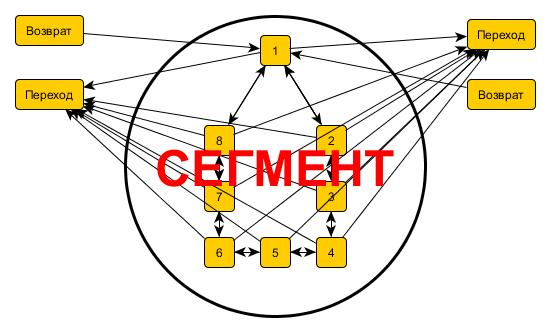
\includegraphics[scale = 0.5]{segment_of_sys_graf.jpg}
	\caption{Сегмент системы состоит из графа состояний.}
	\label{fig:segment_of_sys_graf}
\end{figure}

Каждый сегмент имеет уникальное графическое представление. Два сегмента связанны друг с другом через вершины ''Переход'' и ''Возврат'', где направление перехода от вершины ''Переход'' к вершине ''Возврат''. При переходе от одного сегмента к другому в вершине "Переход" вызываются все необходимые функции (функция завершения выполняемых процессов, функция сохранения актуальных данных, функция очистки выделенной динамической памяти) для завершения работы сегмента. Далее в вершине "Возврат" вызываются все необходимые функции (функции выделения динамической памяти под новые сущности, функция инициализации, функции загрузки информации предыдущей сессии) для загрузки и запуска следующего сегмента (см. рис.\ref{fig:segments_of_sys_graf}).
\begin{figure}[ht]
	\centering
     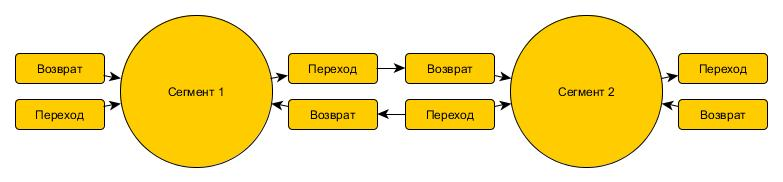
\includegraphics[scale = 0.5]{segments_of_sys_graf.jpg}
	\caption{Связи двух сегментов.}
	\label{fig:segments_of_sys_graf}
\end{figure}

Каждый сегмент уникален и отвечает за свое графическое окно(окно ввода данных клиента, окно тренировки, окно измерения и т.д.), связи сегментов эквиваленты переходам между окнами (см. рис.\ref{fig:segment_sys_graf}).
\begin{figure}[ht]
	\centering
     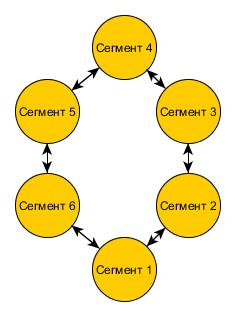
\includegraphics[scale = 0.5]{segment_sys_graf.jpg}
	\caption{Граф связей сегментов.}
	\label{fig:segment_sys_graf}
\end{figure}

\section{Графическая оболочка}

Вся графика была написана на основе библиотеки VGA внутри которой была только попиксельная прорисовка и терминальный способ вывода сообщений.

Графическая оболочка, которая была создана для проекта, это набор созданных форм графического интерфейса, все написанные формы хранятся в библиотеке VGA\_windows. Форма обычна заполняет каким-либо контентом весь экран, контент представляет собой набор объектов класса CntrlSubGroup из библиотеки cntrlsubgroup (см. Приложение В), есть так же цветовые стили, которые хранятся в библиотеке colorsourse. Ниже приведены фотографии, сделанные вовремя работы системы(см. рис.\ref{fig:Graphic_interface_1},\ref{fig:Graphic_interface_2},\ref{fig:Graphic_interface_3})


\begin{figure}[ht]
	\centering
     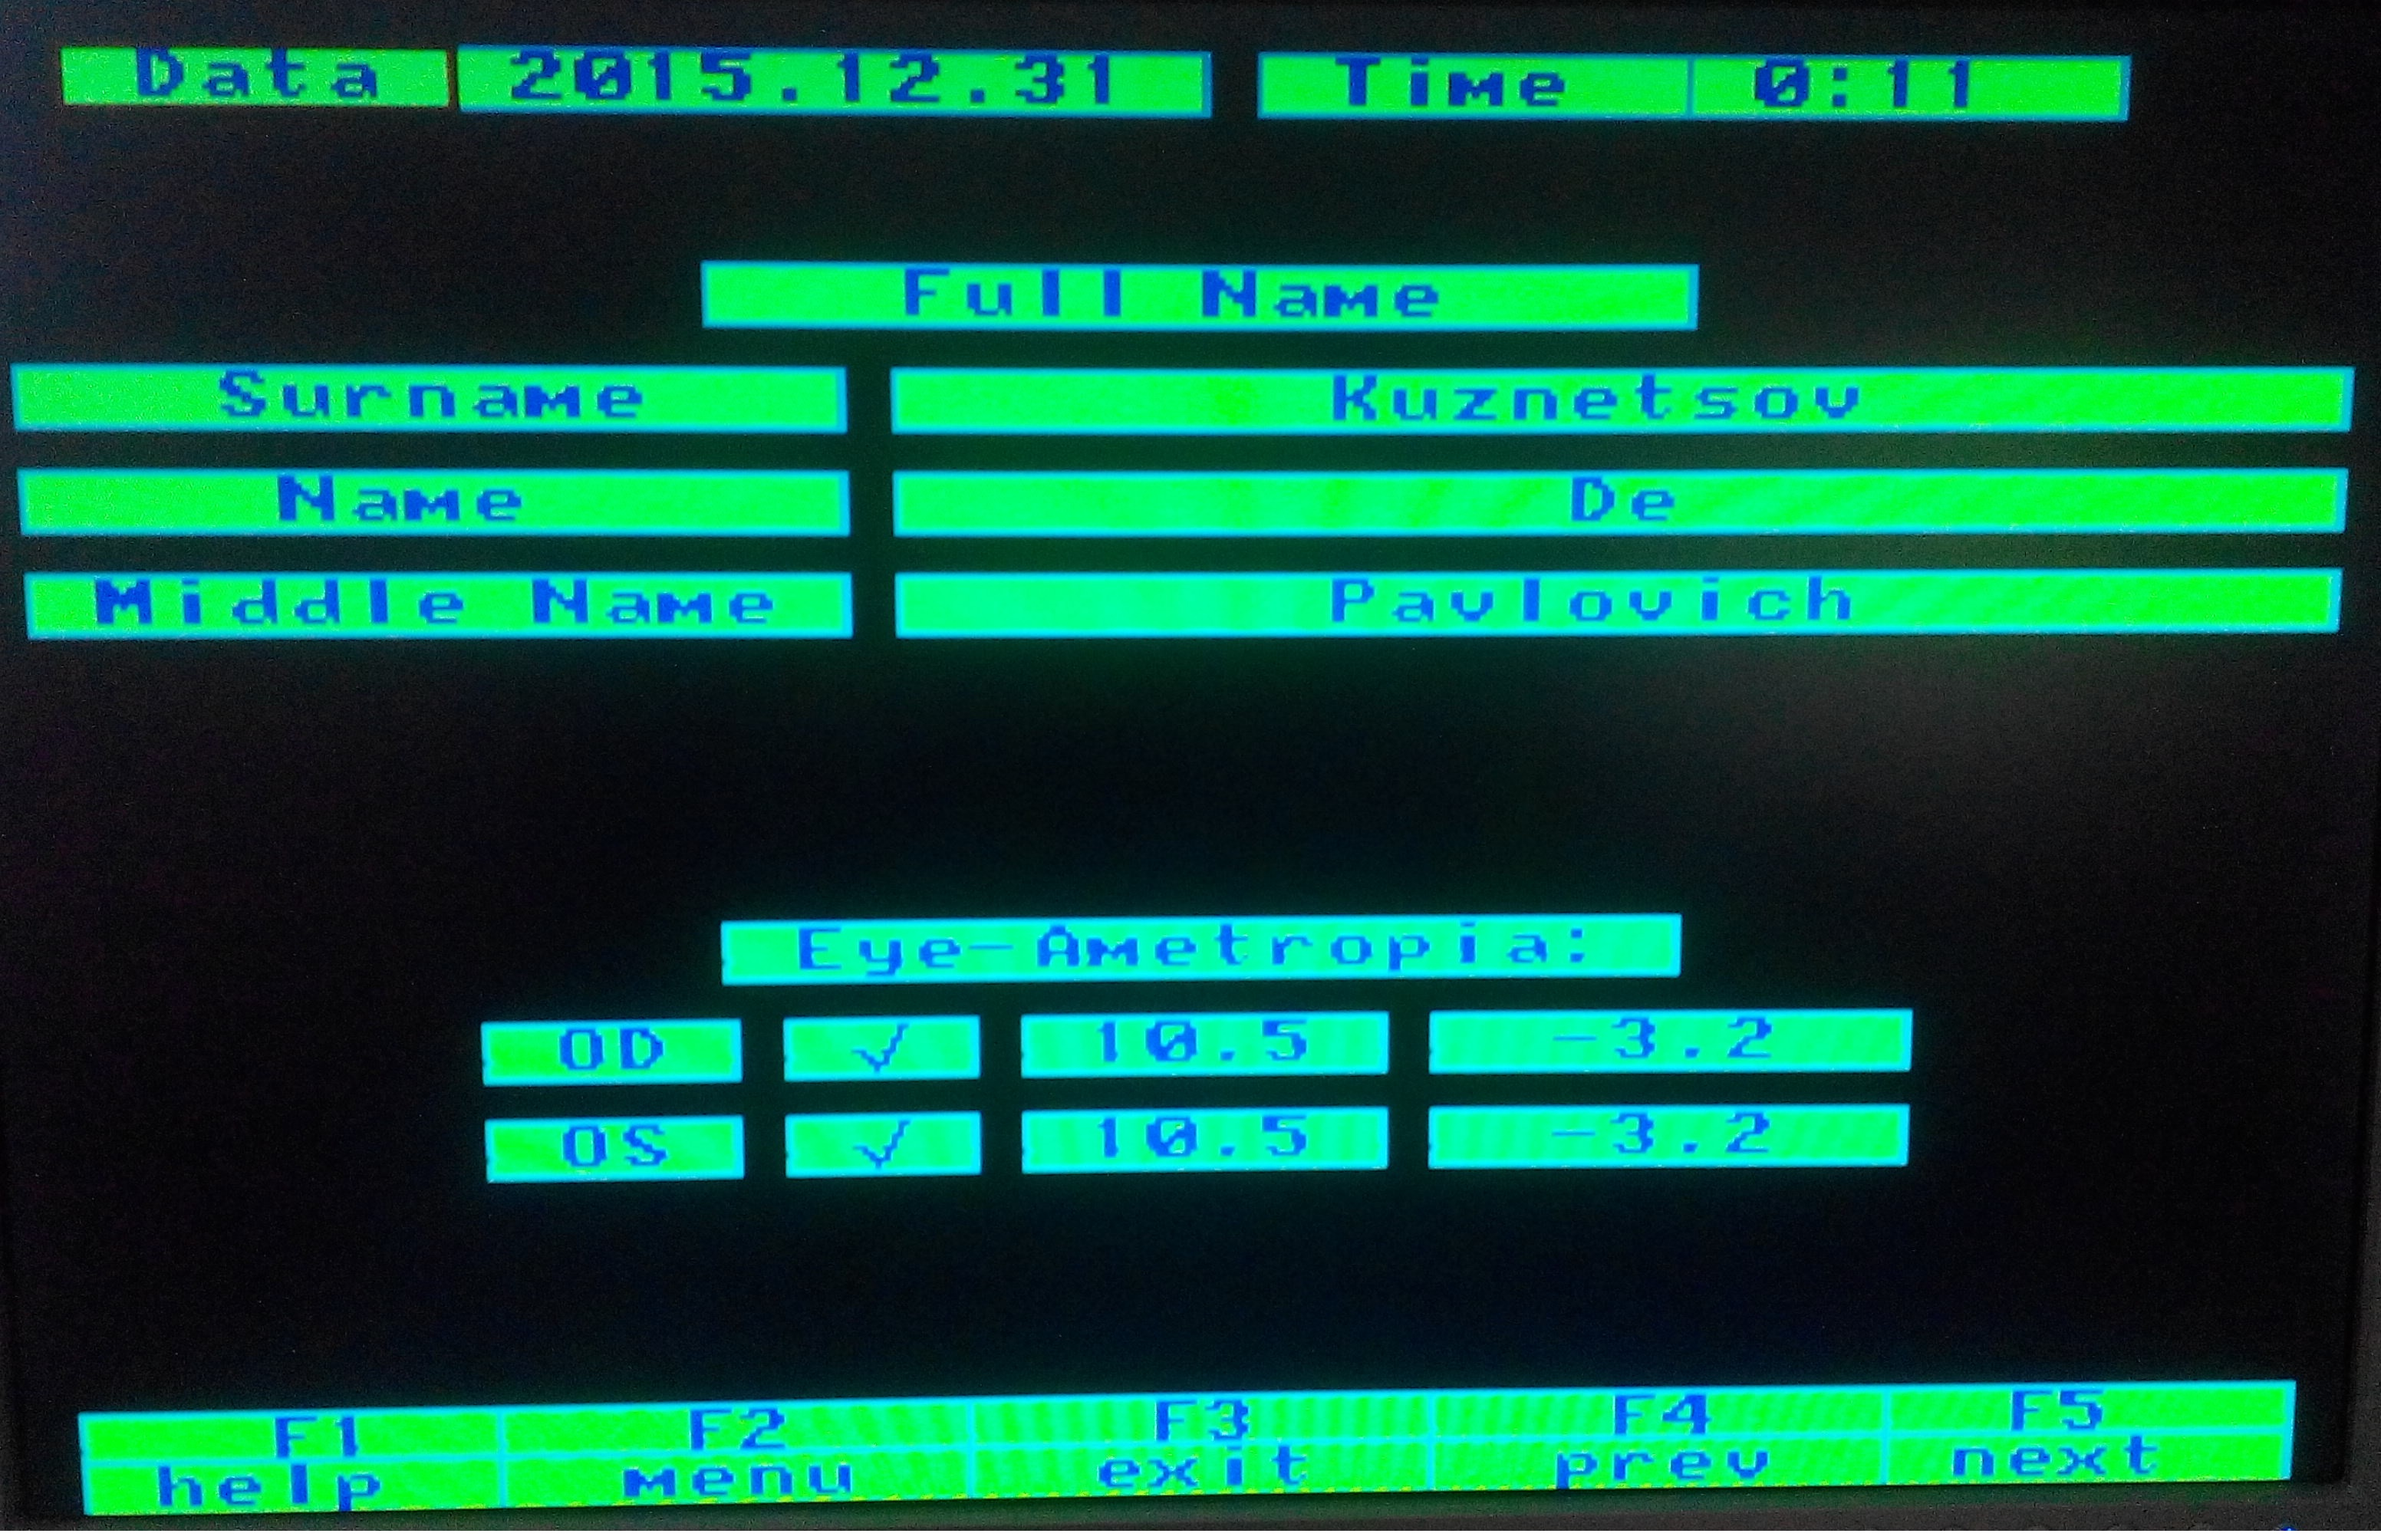
\includegraphics[scale = 0.06]{Graphic_interface_1.jpg}
	\caption{Окно ввода данных клиента 1.}
	\label{fig:Graphic_interface_1}
\end{figure}
\begin{figure}[ht]
	\centering
     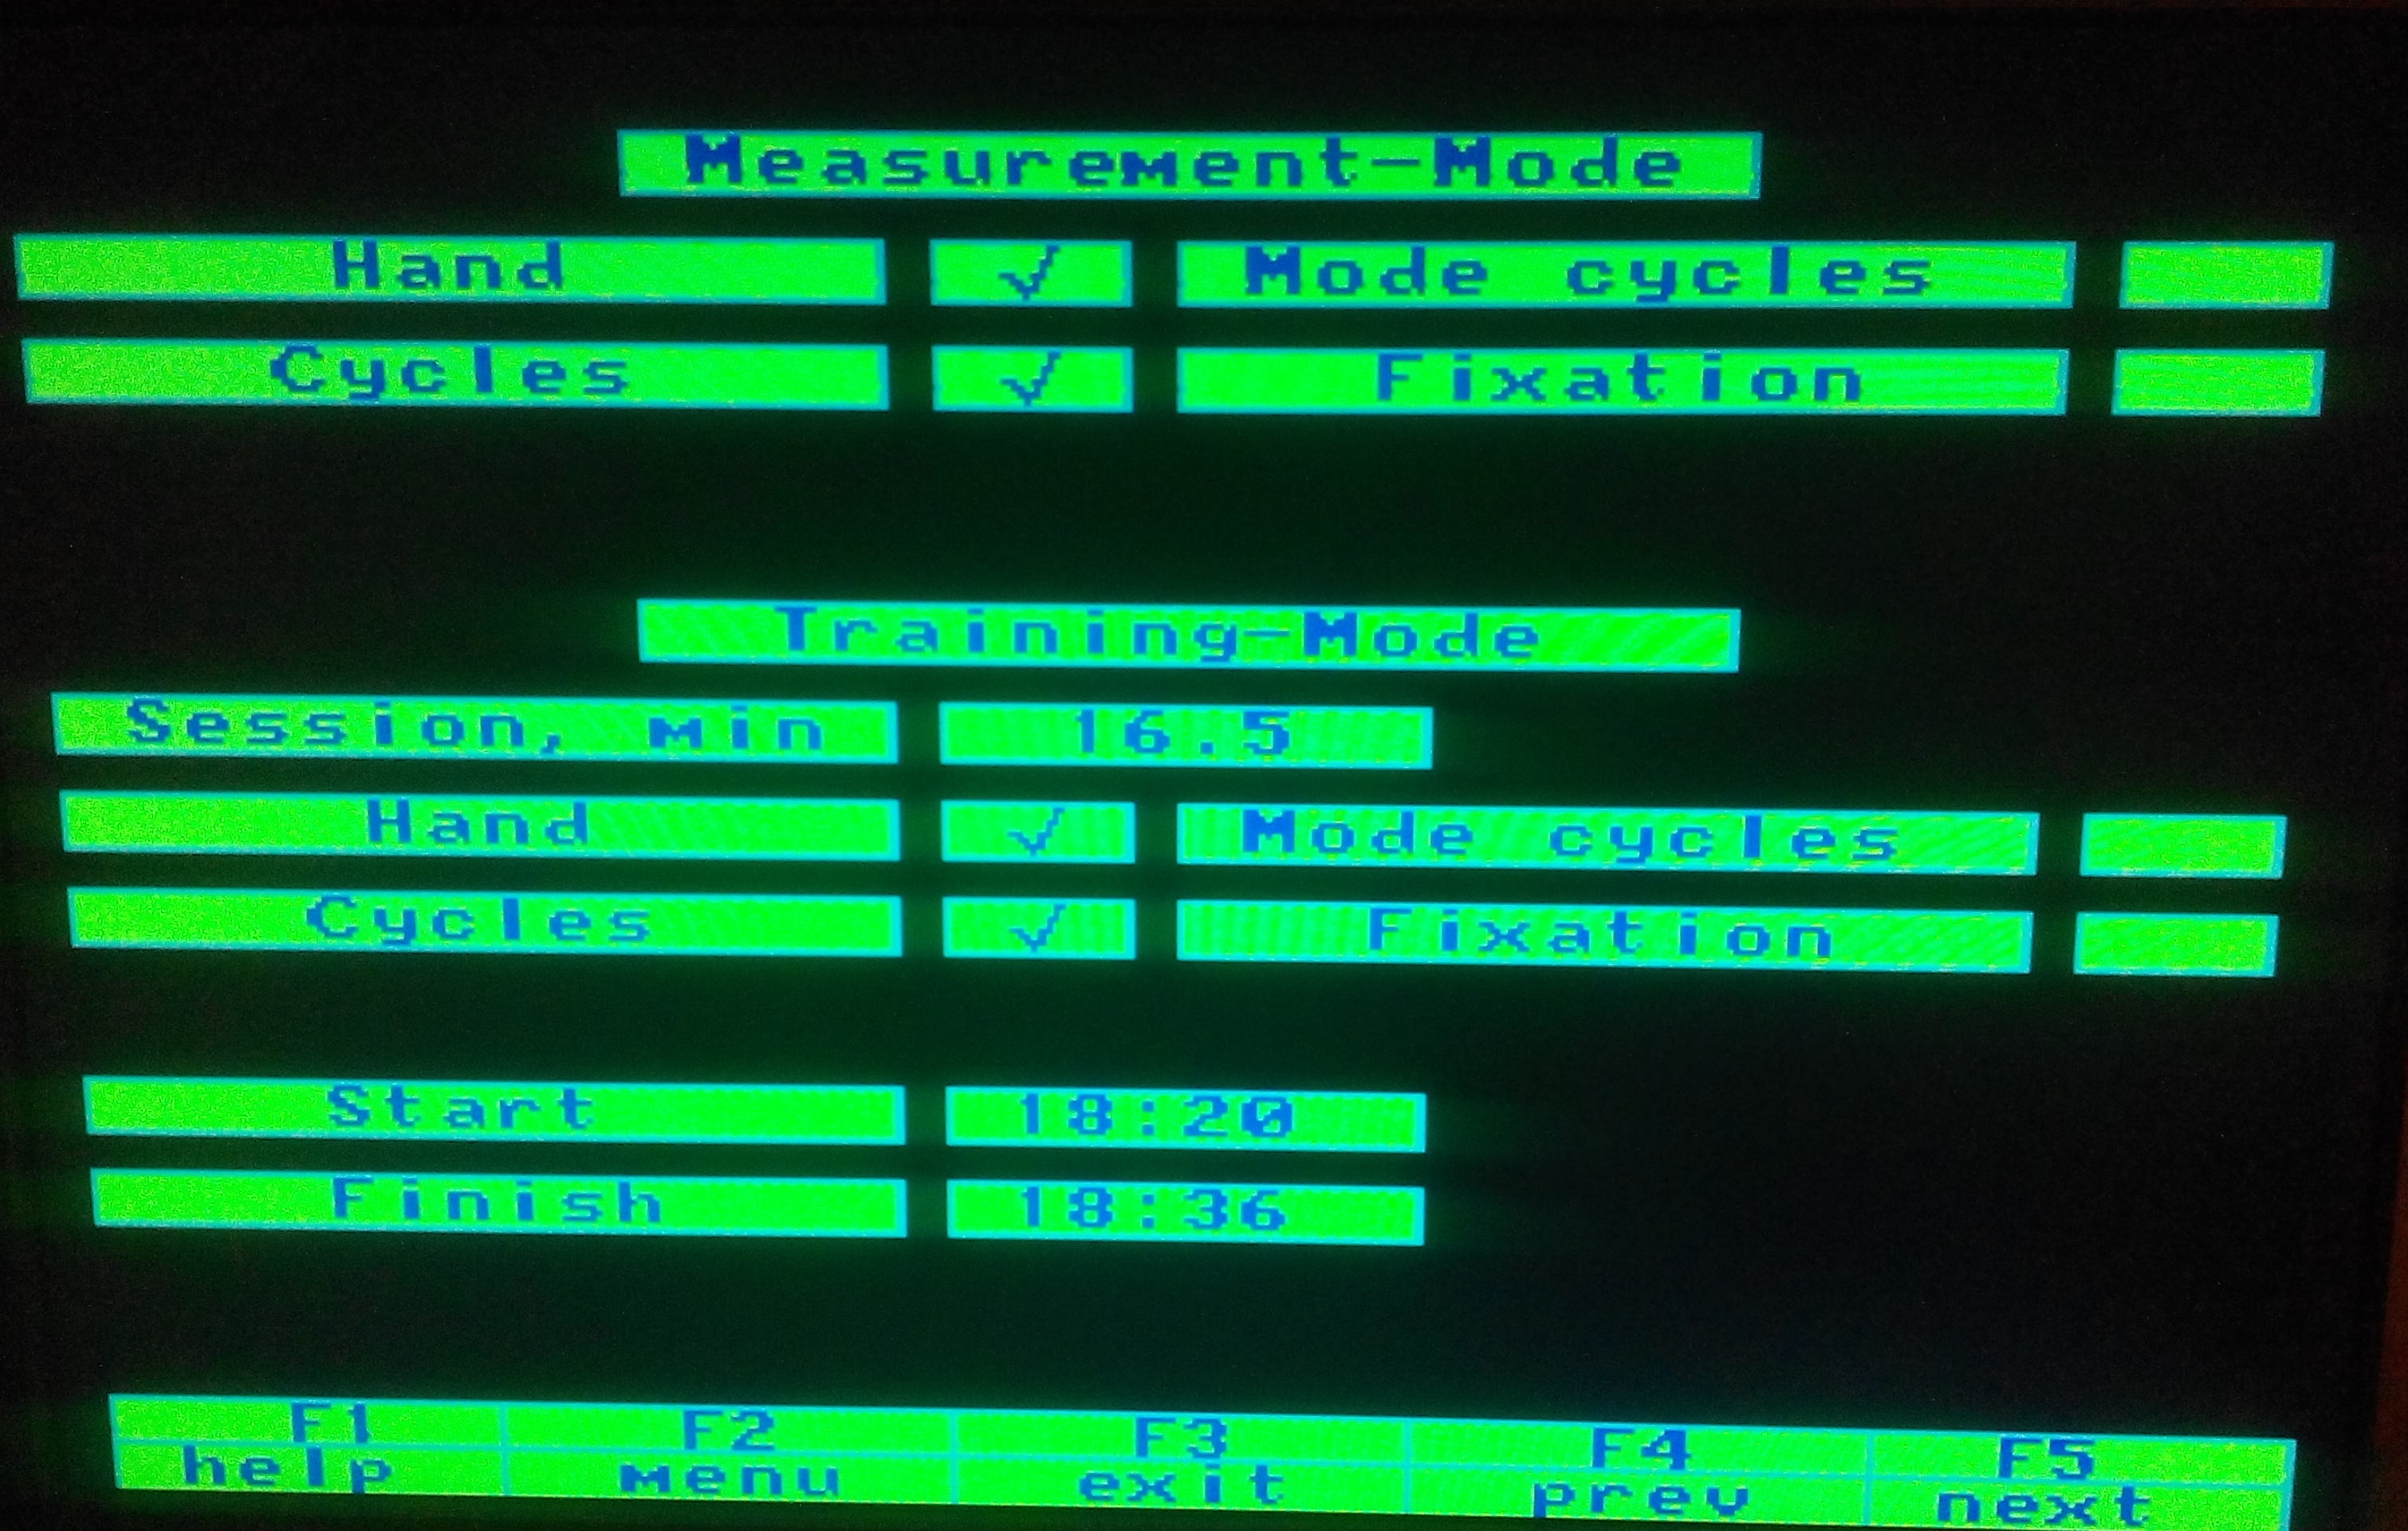
\includegraphics[scale = 0.06]{Graphic_interface_2.jpg}
	\caption{Окно ввода данных клиента 2.}
	\label{fig:Graphic_interface_2}
\end{figure}
\begin{figure}[ht]
	\centering
     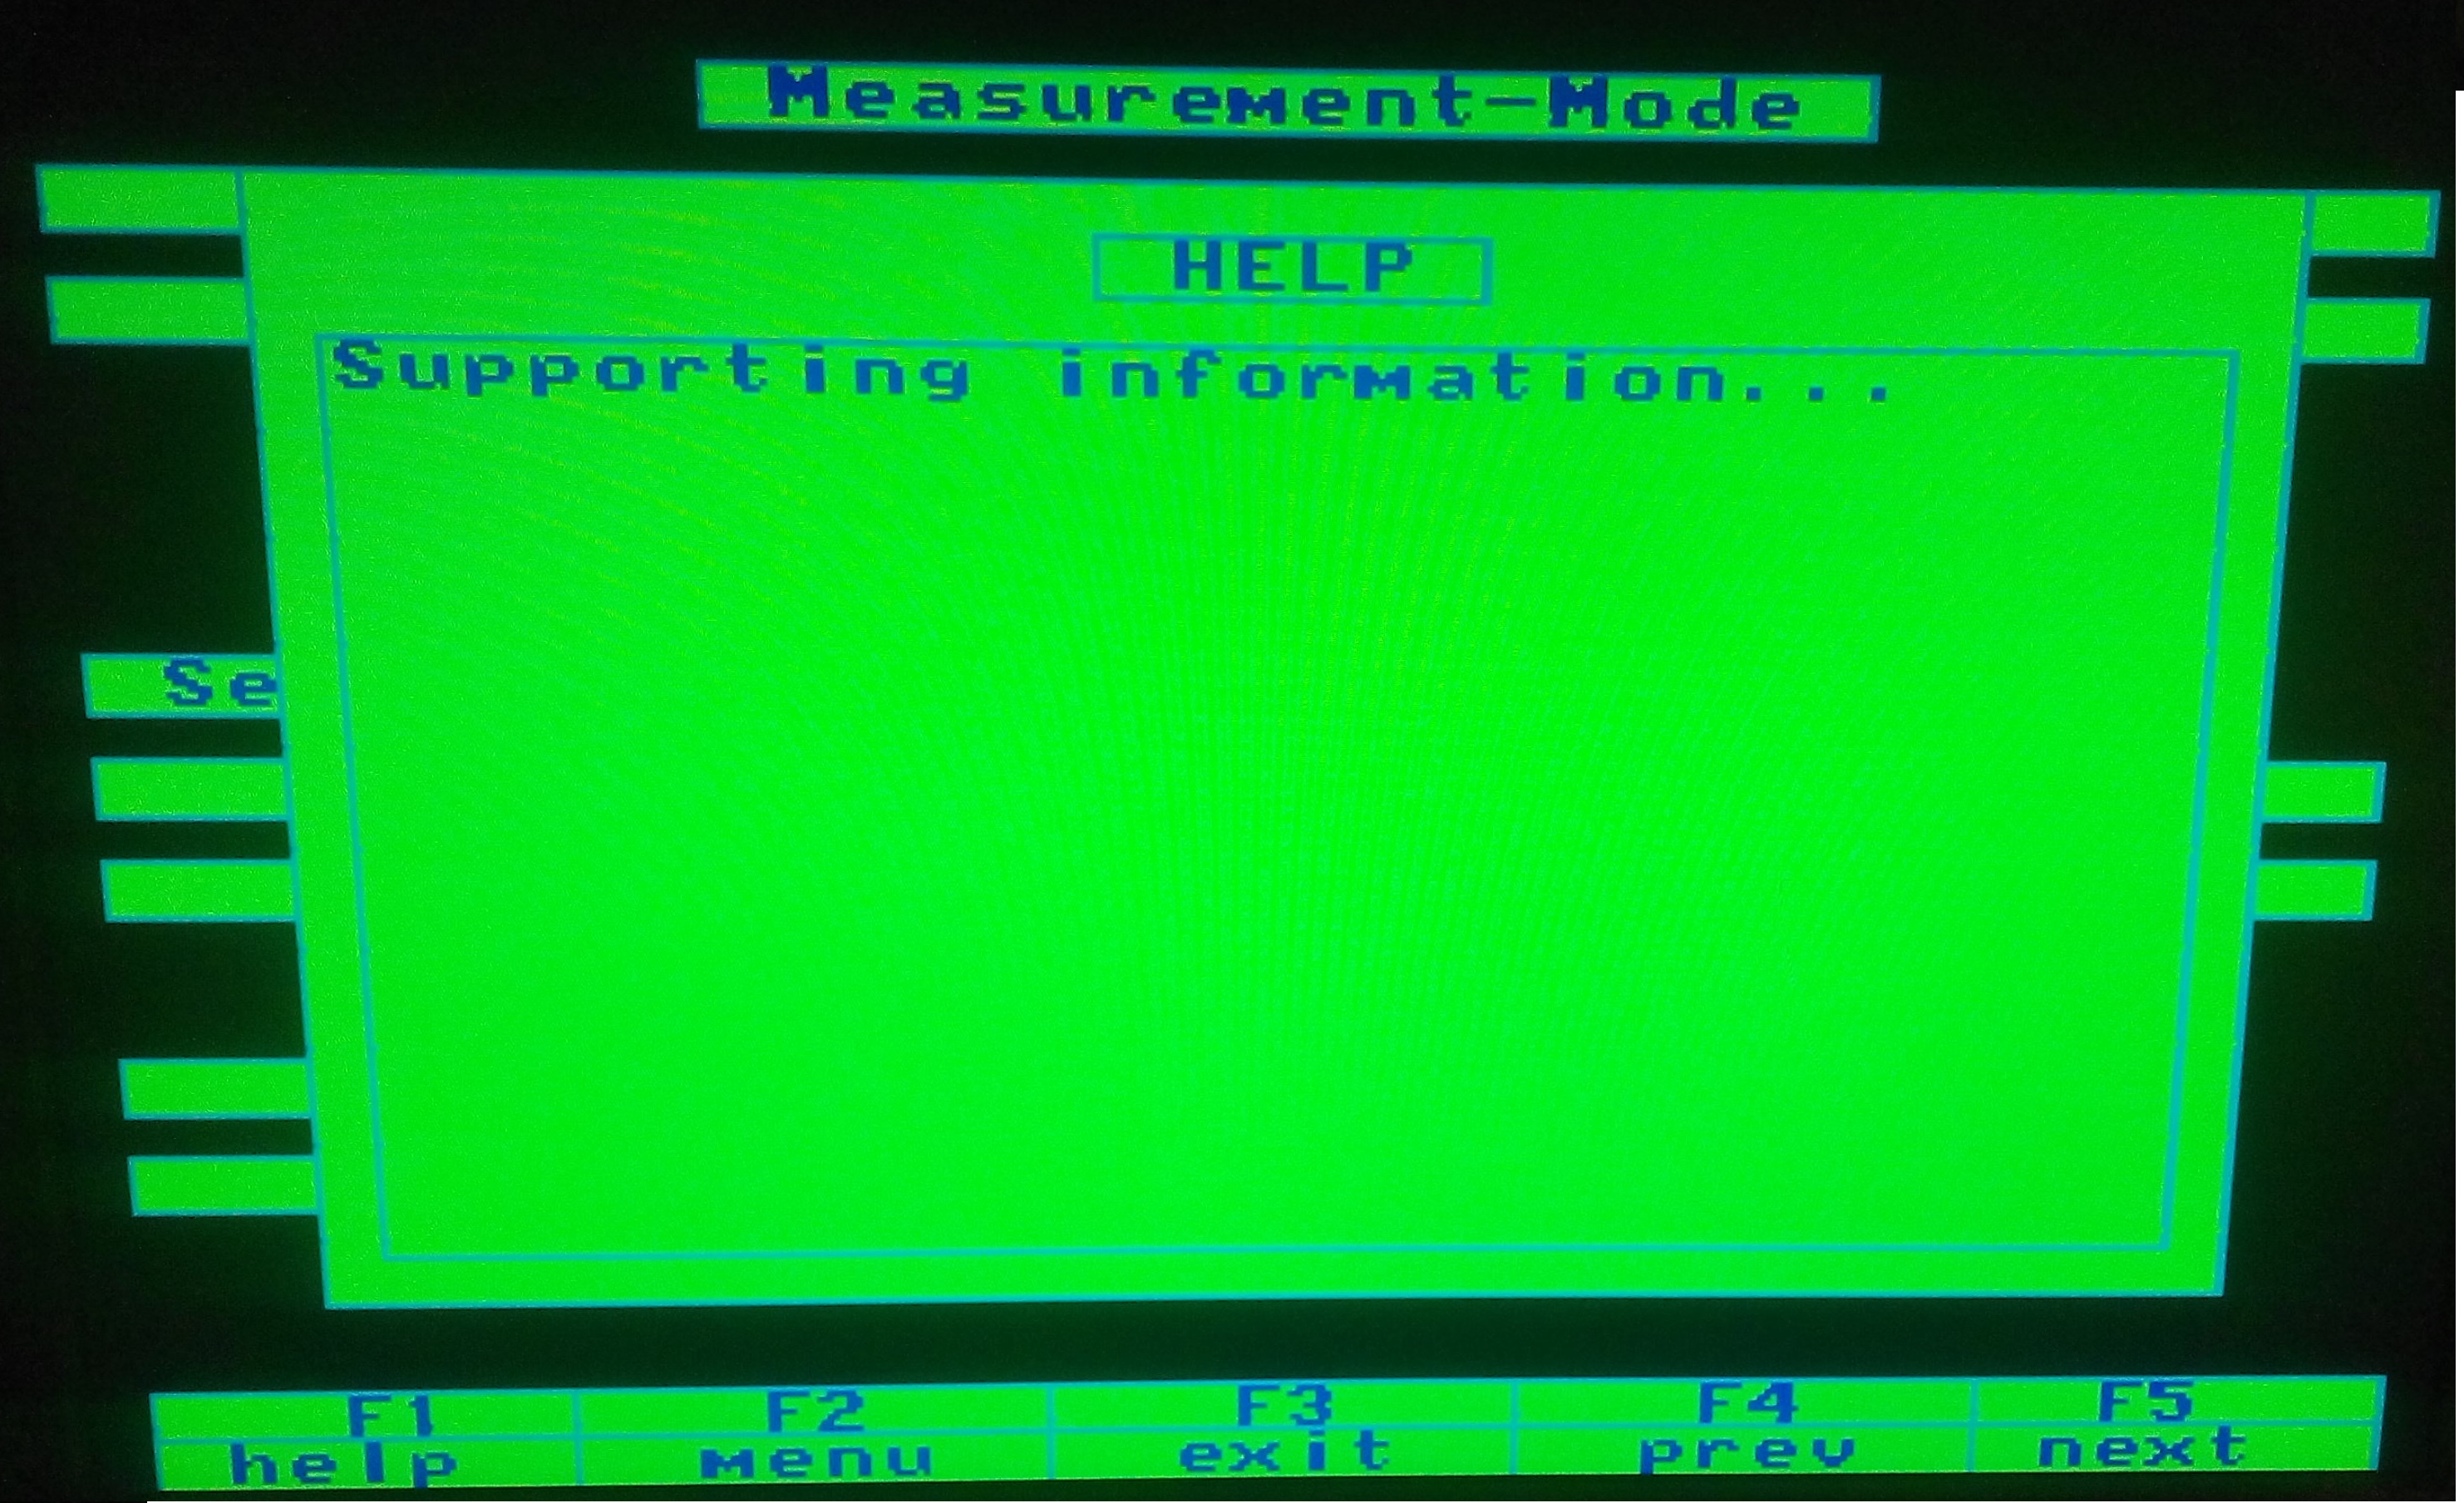
\includegraphics[scale = 0.06]{Graphic_interface_3.jpg}
	\caption{Окно помощи.}
	\label{fig:Graphic_interface_3}
\end{figure}

Представленные снимки показывают стиль с зеленным бэкграундом объектов, цветовой стиль интерфейса можно поменять.

Библиотека VGA была без поддержки русского языка, кодовые страницы для русского пришлось внедрять отдельно, а так же дополнять функцией трансляции, для ввода текста с клавиатуры

\section{Модуль позиционирования}

Модуль управления положением (см. табл.\ref{graf:PositionM}), запускается только при нахождении пользователя в определенном сегменте системы. Запуск начинается с инициализации (определение точки отсчета и возврат на базовую.) Сигналы управления исполняются в следующем приоритете:
\begin{enumerate}
\item сигнал концевого выключателя;
\item клавиатура;
\item энкодер;
\item джойстик.
\end{enumerate}


\begin{figure}[ht]
	\centering
     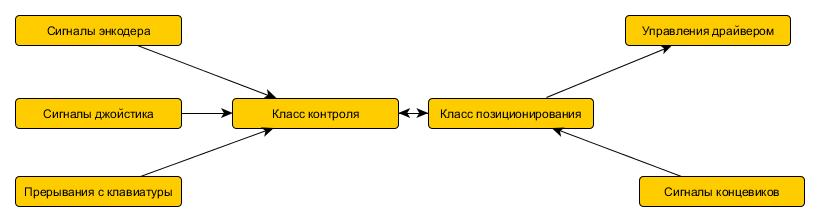
\includegraphics[scale=0.57]{position_module_graf.jpg}
	\caption{Модуль позиционирования.}
	\label{graf:PositionM}
\end{figure}

Этот модуль использует opensource библиотеку KeyBoard и написанные библиотеки:
\begin{itemize}
\item управление двигателем и считывание сигналов с концевого выключателя (A4988);
\item считывание сигналов с джойстика, энкодера обработка прерываний клавиатуры (Keyes\_Sjoys);
\end{itemize}

\section{Модуль внешнего запоминающего устройства}

Базируется на opensource библиотеки SD. Модуль внешнего запоминающего устройства содержит набор функций упрощающих работу с SD картой, например, запись конспекта осмотра больного, чтения из памяти файлов изображения и параметров слайда для модуля визуализации клиента (см. стр. \pageref{page:clientvisialmodule}), сохранение статистики, сохранение постоянных настроек и т.д.


\section{Модуль визуализации клиента}
\label{page:clientvisialmodule} 
Объединяет систему распознавания слайдов и OEL дисплей, он так же как и модуль позиционирование включен в строго определенные сегменты. Для расширенной работы этого модуля необходимо наличие SD карты с информацией по набору слайдов, либо набор файлов изображения которые будет показывать OEL. В случае отсутствия SD система не будет работать в тех режимах, в которых используется содержимое SD.


\begin{figure}[ht]
    \centering
    \begin{subfigure}[b]{0.45\textwidth}
    \centering
        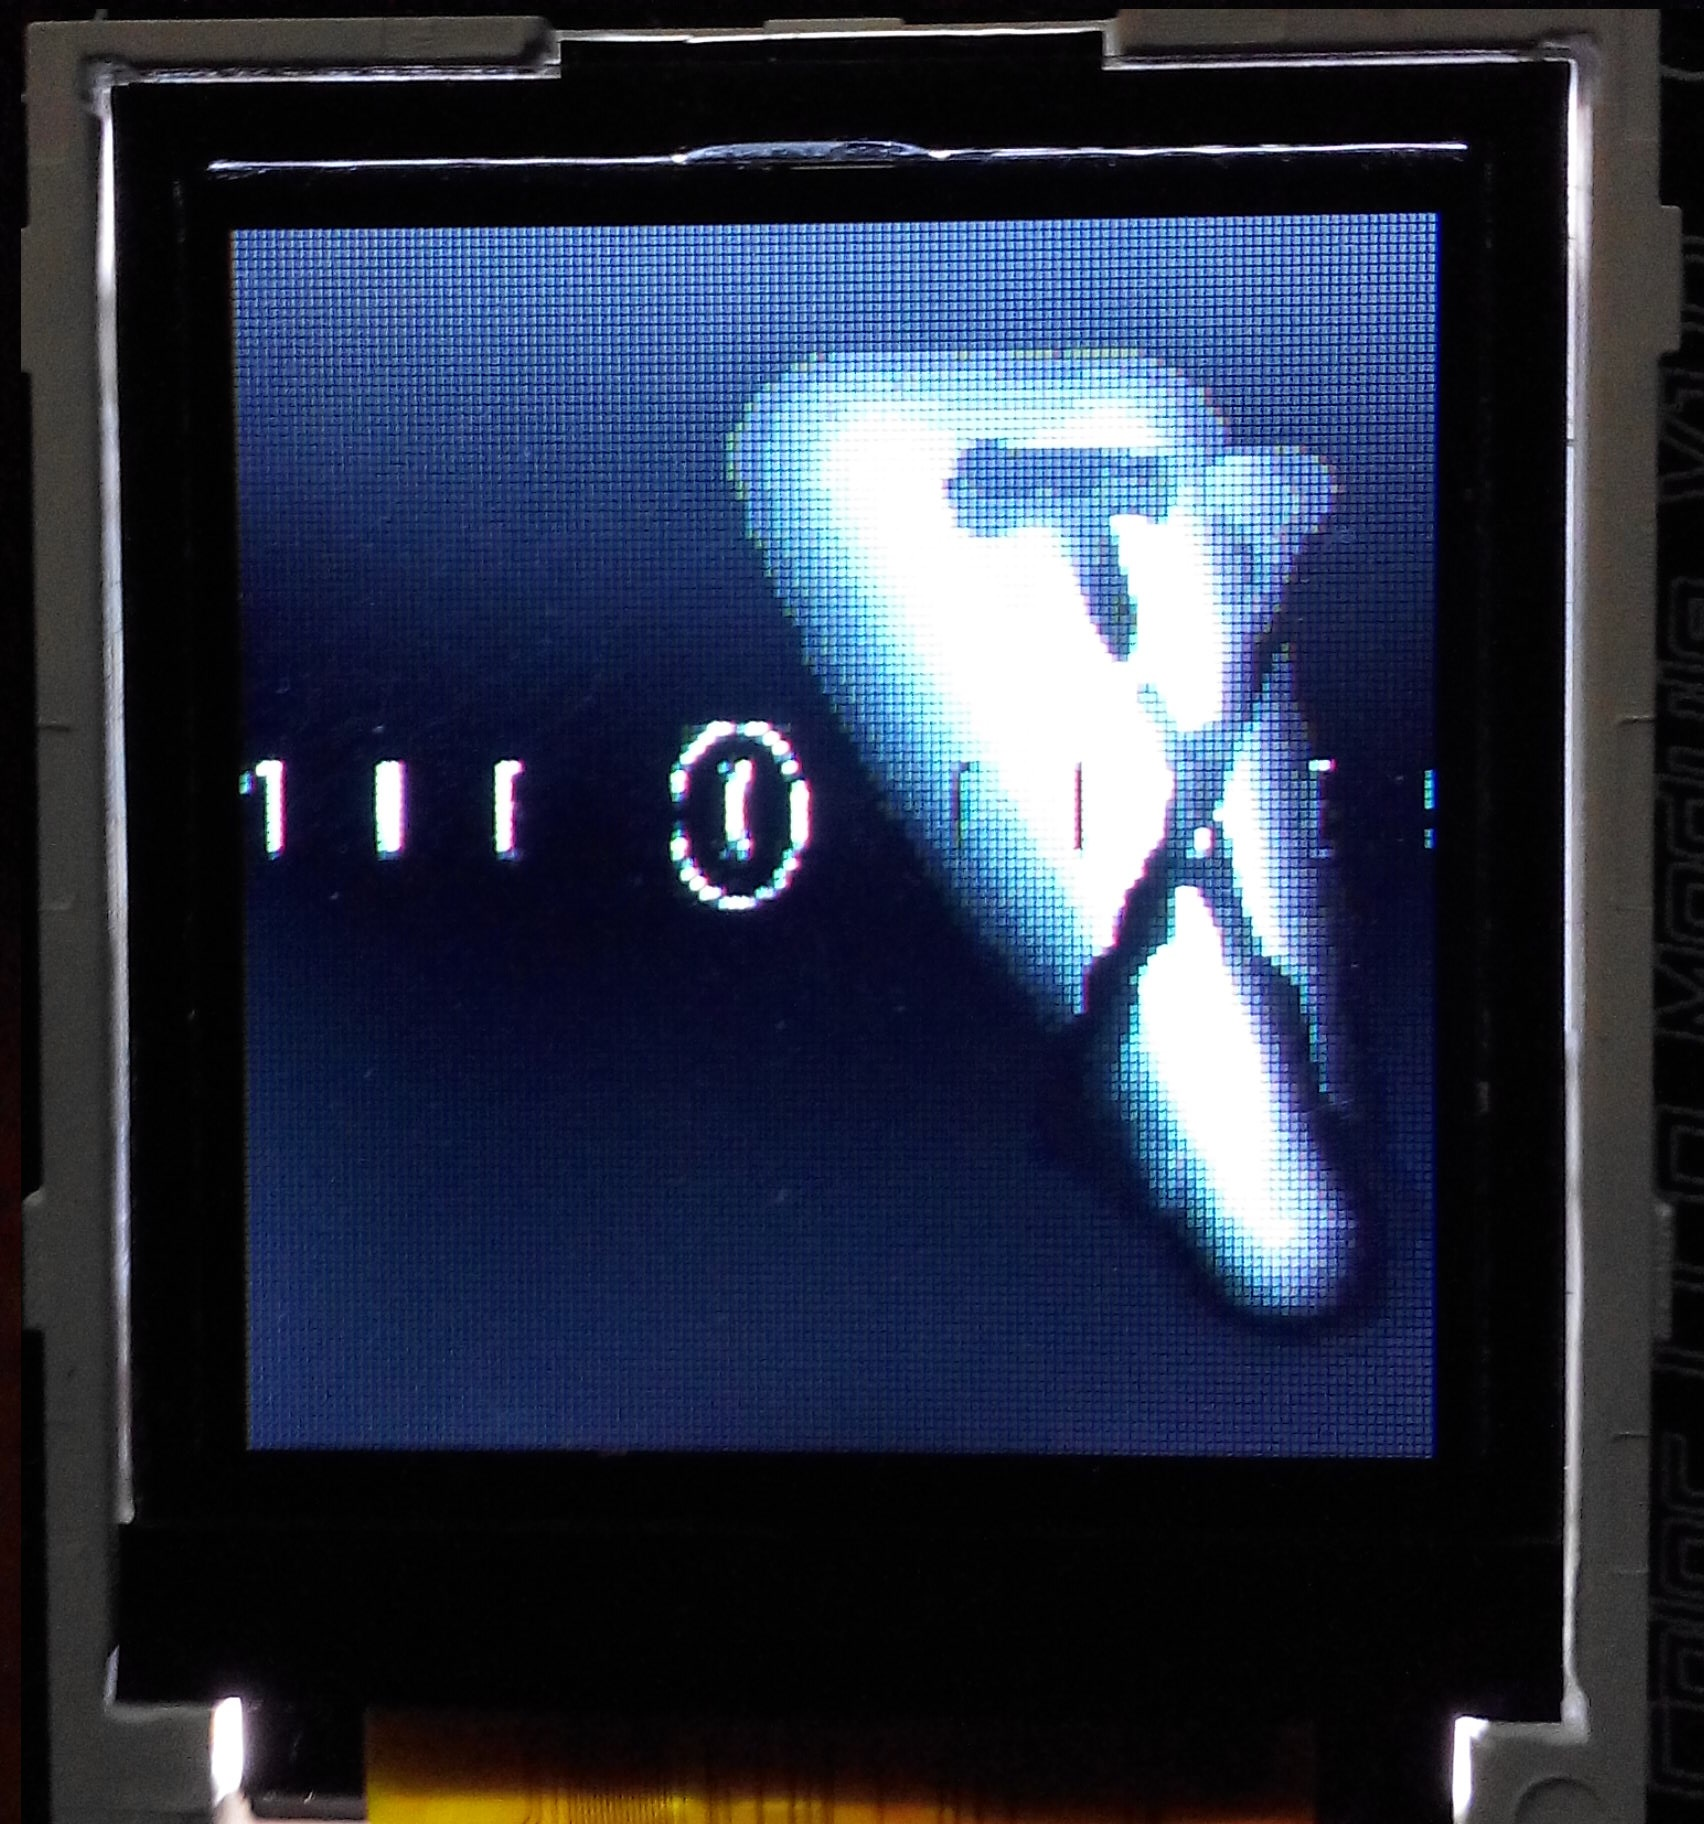
\includegraphics[scale=0.07]{OEL_example1.jpg}
        \caption{}
    \end{subfigure}
    \begin{subfigure}[b]{0.45\textwidth}
    \centering
        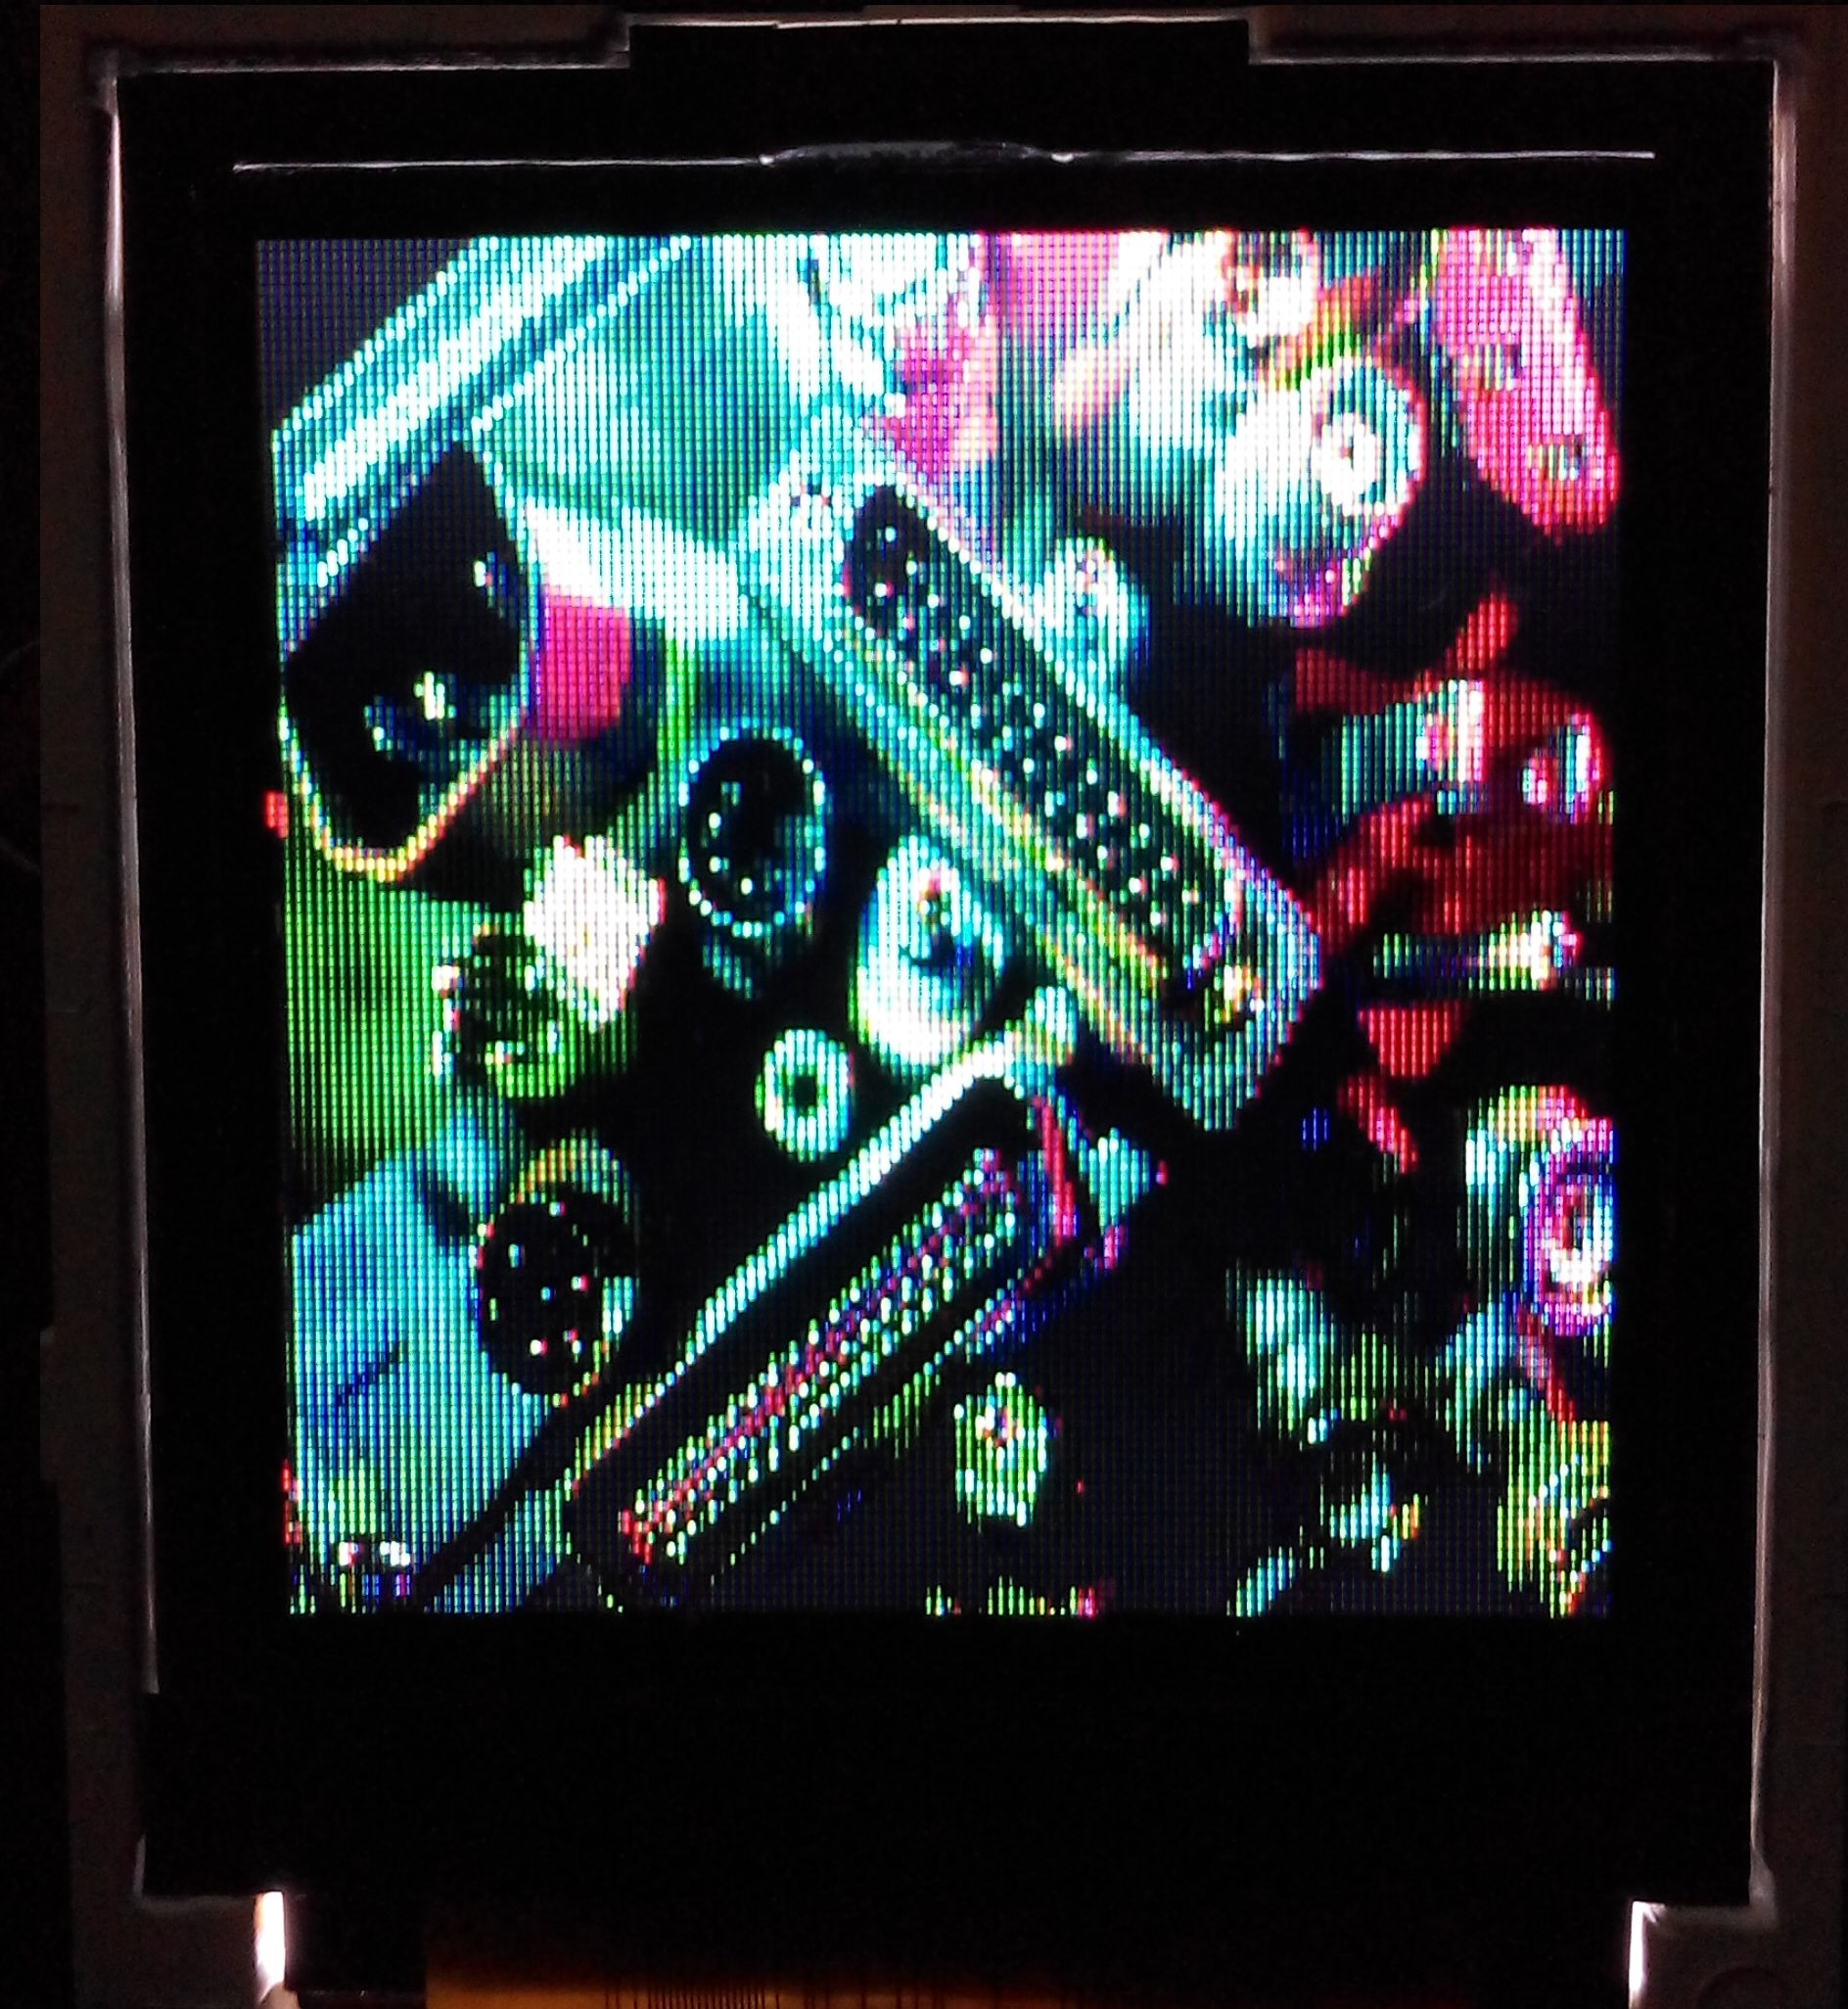
\includegraphics[scale=0.07]{OEL_example2.jpg}
        \caption{}
    \end{subfigure}
    \caption{ (а,б) - загруженные изображения в OEL дисплей.}
    \label{fig:OELDisplExample}
\end{figure}

Инициализация слайда происходит при считывании оптопарами светопроницаемых ячеек, далее определение идентификационного номера, после чего по номеру в библиотеке наборов слайдов (эта библиотека содержит информацию по каждому слайду и расположена на SD карте) определяется расположение тестовых изображений в плоскости слайда. 
Так как слайд стоит перед дисплеем, дисплей может подсвечивать определенные области слайда, тем самым делая видимым определенную картинку, подсвечивание происходит в случайном порядке.
\section{Заключение}
В этой главе была рассмотрена структура и функции ОС. Ограничения контроллера привели к небольшому усложнению системы (создание функций освобождения и выделения памяти под необходимые ресурсы), но благодаря тому, что современные языки программирования, в нашем случае с++, дают возможность абстрагироваться посредством создание классов, шаблонов и т.д., задача была решена. Многие решения были приняты с учетом будущего развития системы.